\documentclass[a4paper,12pt]{article}

\usepackage[T2A]{fontenc} 
\usepackage[utf8]{inputenc}
\usepackage[english,russian]{babel}
\usepackage{listings}
\usepackage[dvips]{graphicx}
\usepackage{indentfirst}
\usepackage{color}
\usepackage{hyperref}
\usepackage{amsmath}
\usepackage{amssymb}
\usepackage{geometry}
\geometry{left=1.5cm}
\geometry{right=1.5cm}
\geometry{top=1cm}
\geometry{bottom=2cm}

\graphicspath{{images/}}

\begin{document}
\sloppy

\lstset{
	basicstyle=\small,
	stringstyle=\ttfamily,
	showstringspaces=false,
	columns=fixed,
	breaklines=true,
	numbers=right,
	numberstyle=\tiny
}

\newtheorem{Def}{Определение}[section]
\newtheorem{Th}{Теорема}
\newtheorem{Lem}[Th]{Лемма}
\newenvironment{Proof}
	{\par\noindent{\bf Доказательство.}}
	{\hfill$\scriptstyle\blacksquare$}
\newenvironment{Solution}
	{\par\noindent{\bf Решение.}}
	{\hfill$\scriptstyle\blacksquare$}


\begin{flushright}
	Кринкин М. Ю. группа 504 (SE)
\end{flushright}

\section{Домашнее задание 10}

\paragraph{Задание 1.} Перечислить ориентированные помеченные графы, а также связные ориентированные помеченные графы.

\begin{Solution}

Число всех помеченных ориентированных графов на $n$ вершинах очевидно равно:
\[
	o_n = 2^{n\cdot \left(n-1\right)}
\]

Далее известно, что если $F\left(x\right)$ - э. п. ф. описывающая все связные графы некоторого вида, то по смыслу композиции э. п. ф. $H\left(x\right) = \exp\left(F\left(x\right)\right)$ описывает все, т. е. связные и не связные, графы того же самого вида.

Теперь если $F\left(x\right) = a_1 x + a_2 \frac{x^2}{2} + a_3 \frac{x^3}{3!} + ...$ и $H\left(x\right) = b_0 + b_1 x + b_2 \frac{x^2}{2} + ...$, то попробуем получить по функции $H\left(x\right)$ функцию $F\left(x\right)$:

\[
	\begin{split}
		& \left(\exp\left(F\left(x\right)\right)\right)' = F'\left(x\right) H\left(x\right) = H'\left(x\right) \Leftrightarrow \\
		& \Leftrightarrow b_1 + b_2 x + b_3 \frac{x^2}{2} + ... = \left(a_1 + a_2 x + a_3 \frac{x^2}{2} + ...\right)\cdot\left(b_0 + b_1 x + b_2 \frac{x^2}{2} + ...\right) \Leftrightarrow \\
		& \Leftrightarrow b_{n+1} = \sum_{i=0}^n \binom{n}{i} b_i a_{n-i+1} \Leftrightarrow b_{n+1} = a_{n+1} + \sum_{i=1}^n \binom{n}{i} b_i a_{n-i+1} \Leftrightarrow \\
		& \Leftrightarrow a_{n+1} = b_{n+1} - \sum_{i=1}^n \binom{n}{i} b_i a_{n-i+1}
	\end{split}
\]

Таким образом, если нам известны коэффициенты $b_n = 2^{n\cdot\left(n-1\right)}$, то и звестны и коэфициенты искомой э. п. ф. для помеченных ориентированных связных графов:
\[
	a_{n+1} = 2^{n\cdot\left(n+1\right)} - \sum_{i=1}^{n} \binom{n}{i} 2^{i\cdot\left(i-1\right)} a_{n-i+1}
\]

осталось определть начальные условия $a_1 = 1$.
\end{Solution}

\paragraph{Задание 2.} Перечислить неориентированные помеченные графы на $n$ вершинах, в которых степень любой вершины равна двум (так называемые 2-регулярные графы).

\begin{Solution}
Связанный 2-регулярный неориентированный граф - простой цикл. Число помеченных простых циклов считается легко:
\[
	c_n = \frac{\left(n-1\right)!}{2}
\]

Теперь пусть граф не связанный, значит он распадается на несколько простых циклов. Будем обозначать число несвязных 2-регулярных помеченных графов на $n$ вершинах, через $l_n$, тогда выведем реккурентную формулу.

Все 2-регулярные помеченные графы, на $n+1$ вершинах распадаются на два класса:

\begin{enumerate}
\item Класс, в котором вершина $n+1$ находится в цикле длинны 3. Число способов составить цикл длинны 3 с вершиной $n+1$ равно $\binom{n}{2} = \frac{n\cdot\left(n-1\right)}{2}$, остальные $n-1$ вершину можно организовать в 2-регулярные помеченный граф $l_{n-1}$ способами.

\item Класс, в котором вершина $n+1$ входит в цикл длинны $\ge 4$. Удалив из цикла в который входит вершина $n+1$ саму $n+1$ и замкнув цикл получим 2-регулярный помеченный граф на $n$ вершинах, и обратно, добавив в некоторый цикл графа на $n$ вершинах получим граф на $n+1$ вершине, в котором $n+1$ вершина входит в цикл длинны $\ge 4$. В графе на $n$ вершинах, ровно $n$ ребер, и добавить к ним $n+1$ вершину соответственно можно $n$ способами.
\end{enumerate}

собираем все вместе:

\[
	l_{n+1} = l_{n-1} \frac{n\cdot\left(n-1\right)}{2} + l_n n
\]

Начальные условия $l_2 = 0, l_3 = \frac{3!}{2} = 3$

\end{Solution}

\paragraph{Задание 3.} Перечислить все помеченные эйлеровы графы, т. е. связные графы, в которых любая вершина имеет четную степень (на прошедшем занятии была пройдена половина пути - было найдено число помеченных графов с четными вершинами; осталось выбрать из них количество односвязных компонент). Сосчитать, сколько эйлеровых помеченных графов существует на пяти вершинах; дать их описание (нарисовать различные непомеченные графы и указать, сколько способов существует разметить их вершины).

\begin{Solution}
Нам известно, что число помеченных графов на $n$ вершинах, в которых все вершины имеют четную степень равно:

\[
	2^{\binom{n-1}{2}}
\]

Тогда пользуясь формулой из первого задания получим число связных графов, в которых каждая вершина имеет четную степень, т. е. эйлеровых графов без свободных вершин на $n+1$ вершине ($l_{n+1}$):

\[
	l_{n+1} = 2^{\binom{n}{2}} - \sum_{i=1}^{n} \binom{n}{i} 2^{\binom{i-1}{2}} l_{n-i+1}
\]
в качестве начальных условий можно взять $l_1 = 1, l_2 = 0$.

\begin{figure}[h]
\begin{center}
\noindent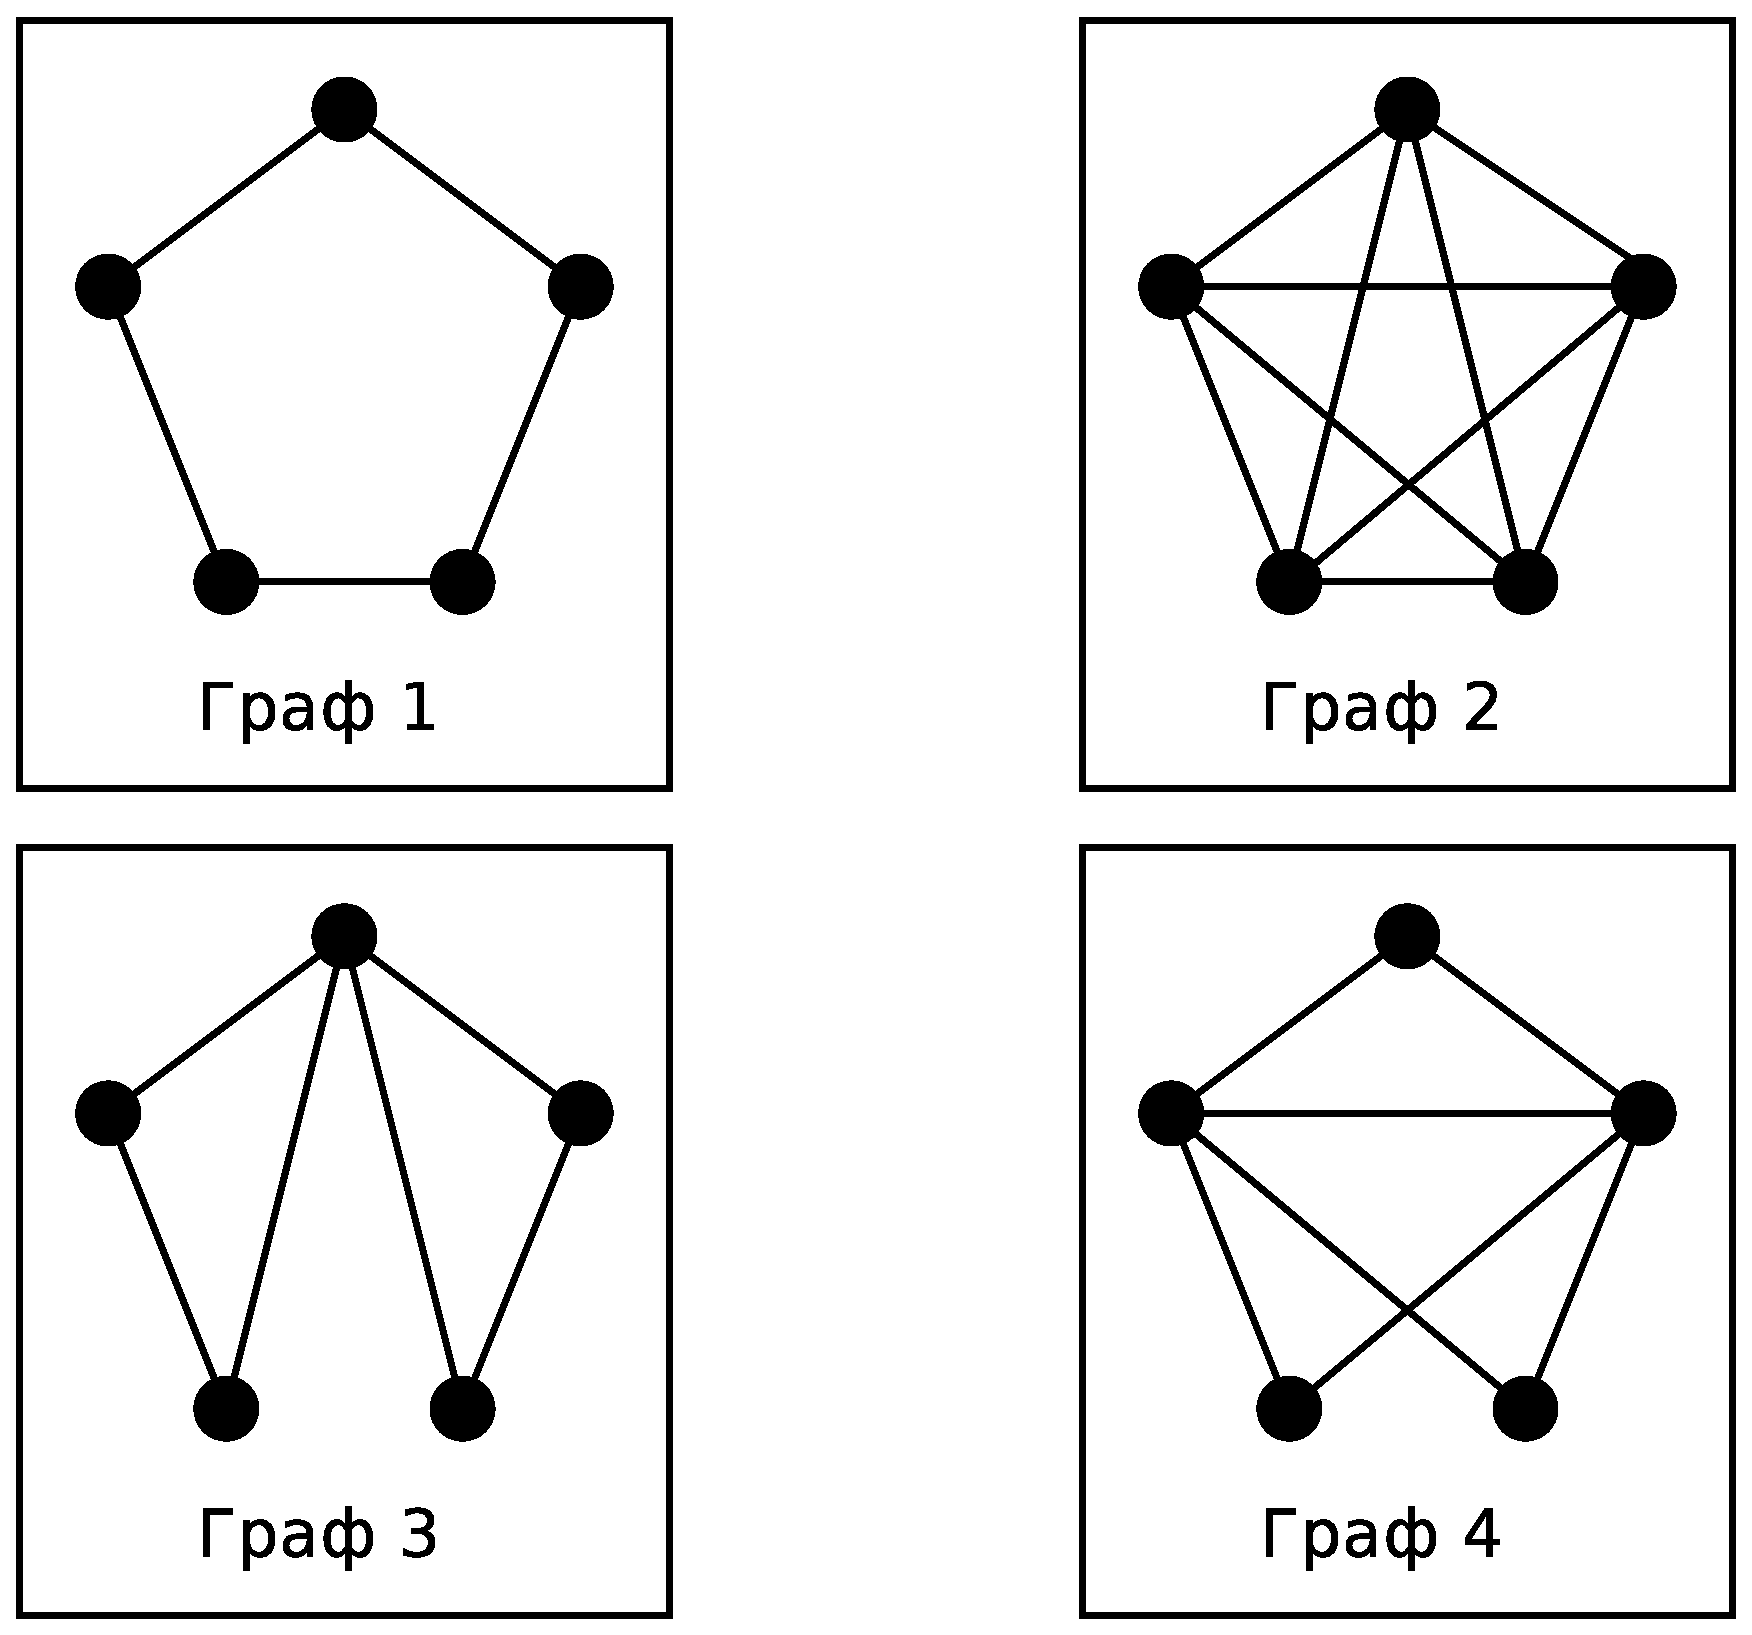
\includegraphics[width=0.4\linewidth]{graphs}
\caption{Эйлеровы графы на 5 вершинах}
\label{img::graphs}
\end{center}
\end{figure}

Существует 4 структурно различных эйлеровых связных графа на пяти вершинах, все они приведены на рис. \ref{img::graphs}

Граф 1 можно пометить $\frac{4!}{2} = 12$ способами, граф 2 можно пометить всего одним способом, граф 3 можно пометить $5 \cdot 3 = 15$ способами, пометить 4 граф можно $\binom{5}{2} = 10$, в сумме дет требуемые 38 вариантов.
\end{Solution}

\paragraph{Задание 4.} Завершить начатое на занятии доказательство теормеы Кэлли о количестве помеченных деревьев на $n$ вершинах, опирающееся на использование кода Прюфера.

\begin{Solution}
Алгоритм получения последовательности по помеченному дереву:

\begin{lstlisting}
while |V| > 1
	1. v = min{ v \in V | deg(v) = 1}
	2. code.append neighbor(v)
	3. V.delete(v)
\end{lstlisting}

Такой алгоритм сопоставляет каждому дереву на $n$ вершинах последовательность из $n-1$ числа, при этом в этой последовательности последним числом всегда будет $n$, то есть можно отбросить последнее число и получить последовательность длинны $n-2$.

Обратно по каждой последовательности можно восстановить дерево. Для последовательности длинны 1 это очевидно.
Пусть для всех последовательностей не длиннее $n$ мы можем восстановить дерево, покажем, что для $n+1$ последовательности это также возможно. Для этого выберем минимальное число $v$ из $\left[n\right]$ отсутствующее в последовательности. Добавим в дерево ребро связывающее $v$ и первое число последовательности. Удалим первое число из последовательности и перенумеруем вершины с номером $>v$, уменьшив номер на единицу. Получили последовательность меньшей длинны.

Получается, что коды Прюфера длинны $n-2$ и деревья на $n$ вершинах помеченные числами из $\left[n\right]$ связаны биекцией. Всего таких последовательностей $n^{n-2}$, а следовательно и число помеченных деревьев на $n$ вершинах равно $n^{n-2}$.
\end{Solution}

\paragraph{Задание 5.} С использованием кода Прюфера сосчитать количество различных помеченных деревьев на множестве вершин $\lbrace1, 2, 3, 4, 5, 6, 7\rbrace$, в которых вершины 2 и 3 имеют степень 3, вершина 5 имеет степень 2, а остальные вершины, как следствие, имеют степень, равную 1.

\begin{Solution}
Так как степень $2$ и $3$ равна 3 и их номера не максимальные возможные, то они встретятся в коде по 2 раза. Вершина 5 обязательно встретится в коде, так как имеет степень 2, а так как весь код должен иметь длину 5, то встретится она там ровно 1 раз, следовательно нужно посчитать количество последовательностей длинны 5, в которых 5 встречается ровно 1 раз, а 2 и 3 по 2 раза:

\[
	5 \cdot 6 = 30
\]
\end{Solution}

\paragraph{Задание 6.} Пусть $f\left(n,r,s\right)$ - число разбиений множества $\left[n\right] = \lbrace1, 2, ..., n\rbrace$, в котором имеется ровно $r$ классов размером 1 и ровно $s$ классов размером 2; количество классов размером, большим 2, может быть любым. Построить производящую функцию $F\left(x, y, t\right)$ трех аргументов для этих чисел.

\begin{Solution}
\end{Solution}

\paragraph{Задание 7.} Перечислить количество двудольных помеченных графов.

\begin{Solution}
Рассмотрим сначала правильно 2-раскрашенные помеченные графы. Если в графе $n$ вершин, то разбить его на 2 доли можно $\sum_{i=0}^n \binom{n}{i}$ способами, при каждом таком разбиении ребра можно провести $2^{i\cdot\left(n-i\right)}$ способами, итого число 2-раскрашенных помеченных графов равно:

\[
	g_n = \sum_{i=0}^n \binom{n}{i} 2^{i\cdot\left(n-i\right)}
\]

Э. п. ф. для таких графов обозначим $G\left(x\right) = \sum_{i=0}^{\infty} g_n \frac{x^i}{i!}$. Далее обозначим число связных двараскрашенных графов через $С\left(x\right)$, тогда справедливо соотношение:

\[
	G\left(x\right) = \exp\left(C\left(x\right)\right) \Leftrightarrow \ln G\left(x\right) = C\left(x\right)
\]

Каждому связному двудольному помеченному графу соответствует 2 связных двурскрашенных помеченных графа, поэтому для двудольных связных графов имеем производящую функцию:

\[
	\tilde C\left(x\right) = \frac{1}{2} \ln C\left(x\right)
\]

Для всех двудольных графов тогда получаем:

\[
	\tilde G\left(x\right) = \exp\left(\frac{1}{2} \ln C\left(x\right)\right) = \sqrt{C\left(x\right)} = \sqrt{\sum_{n=0}^{\infty} g_n \frac{x^n}{n!}}
\]
\end{Solution}

\paragraph{Задание 8.} Рассмотрим $n$-элементное множество, $n \ge 2$ (тут вероятно опечатка, так как дальше рассматривается число $t\left(1\right)$, т. е. всетаки $n \ge 1$). Разобьем его по крайней мере на два блока. Затем каждый блок состоящий из более чем одного элемента, также разобьем по крайней мере на два блока. Продолжая процесс, получим, что в конце каждый блок будет состоять из одного элемента. Указанная процедура называется полным разбиением $n$-множества. Очевидно, что любое полное разбиение пожно представить в виде дерева, в котором достаточно пометить $n$ числами только листья. Пусть $t\left(n\right)$ - число таких полных разбиений.

\begin{itemize}
\item а) Убедиться, что $t\left(1\right) = 1$, $t\left(2\right) = 1$, $t\left(3\right) = 4$, $t\left(4\right) = 26$

\item б) Доказать, что экспоненциальная производящая функция $F\left(x\right)$ для чиел $t_n$ удовлетворяет следующему уравнению:

\[
	\exp\left(F\left(x\right)\right) = 2 F\left(x\right) - x + 1
\]

\item в) Доказать, что в случае разбиения каждого блока, содержащего более чем один элемент, ровно на два блока (т. н. полное двоичное разбиение $n$-множества), экспоненциальная производящая функция $F_2\left(x\right)$ для чисел $b_n$ таких разбиений удовлетворяет равнеству:

\[
	\frac{1}{2} F_2\left(x\right)^2 = F_2\left(x\right) - x
\]

\item г) Получить из этого уравнения следующее явное выражение для чисел $b_n$:

\[
	b_n = 1\cdot 3 \cdot 5 ... \cdot \left(2n - 3\right)
\]
\end{itemize}

\begin{Solution}
Пункт а). Для $t\left(1\right)$ и $t\left(2\right)$ очевидно. Для $t\left(3\right)$ возможны следующие варианты, на первом шаге множество разбивается на 3 элемента, или на первом шаге множество разбивается на два блока (по 2 и по 1 элементу). Разбить на 3 блока 3-множество можно только 1 способом, а на 2 блока 3, всего получае 4 варианта.

Для $t\left(4\right)$ можно уже записать формулу:
\[
	t\left(4\right) = t\left(1\right)\cdot t\left(1\right)\cdot t\left(1\right)\cdot t\left(1\right) + 4 t\left(1\right)t\left(3\right) + 3 t\left(2\right)t\left(2\right) + 6 t\left(2\right) t\left(1\right) t\left(1\right) = 1 + 16 + 3 + 6 = 26
\]

Пункт б). По смыслу композиции э. п. ф. $\exp\left(F\left(x\right)\right)$ означает разбиение $n$-множества на блоки (в том числе возможен и случай когда $n=0$ и когда $n$-множество разбивается на один блок - само $n$-множество), после чего каждый блок разбивается по алгоритму из задания.

Рассмотрим все возможные варианты разбиения $n$-множества, где $n\ge1$. Рассмотрим два случая, первый когда $n$-множество разбивается на 2 или более блоков, второй случай - вырожденное разбиение на 1 блок.

Каждому разбиению первого вида соответсвует полное разбиение $n$-множества, таким образом число способов проделать такое разбиение описывается э. п. ф. $F\left(x\right)$. Число способов проделать вырожденное разбиение (второй случай), также описывается э. п. ф. $F\left(x\right)$.

Кроме того, случай $n = 1$ одновременно порождает вырожденное разбиение и подходит под алгоритм полного разбиения, т. е. посчитан 2 раза. Число способов полного разбиение множества из 1 элемента равно 1, т. е. необходимо отнять $x$. А также с учетом того, что экспонента э. п. ф. имеет нулевым членом 1, которая отсутсвует в $F\left(x\right)$ то получаем требуемую формулу:

\[
	\exp\left(F\left(x\right)\right) = F\left(x\right) + F\left(x\right) - x + 1
\]

Пункт в). Рассмотрим квадрат э. п. ф. $F_2\left(x\right)$. $n$-ый член такого квадарата имеет своим коэффициентом:

\[
	f_n = \sum_{i=0}^n \binom{n}{i} b_i b_{n-i}
\]

Этому выражению нетрудно придать смысл. Оно равносильно количеству способов выбрать некоторое число элементов из $n$-множества и совершить над ними полное двоичное разбиение, а также совершить такое разбиение над невыбранными элементами. При этом, если положить, что выбранные и не выбранные элементы равносильны, то каждое такое разбиение учитывается в сумме 2 раза, т. е. получаем новую формулу:

\[
	\tilde f_n = \frac{1}{2} \sum_{i = 0} ^n \binom{n}{i} b_i b_{n-i}
\]

Очевидно, что для $n$-множества, в котором $n\ge2$, такое комбинаторное действие совпадает с полным двоичным разбиением, для $n=1$ такое комбинаторное действие нельзя совершить, а значит получаем требуемое соотношение:

\[
	\frac{1}{2} F_2\left(x\right)^2 = F_2\left(x\right) - x
\]

Пункт г). Найдем выражение для $F_2\left(x\right)$ из соотношения выше:

\[
	F_2\left(x\right) = 1 \pm \sqrt{1 - 2x}
\]

Оставим пока выбор правильного знака, найдем вид $\sqrt{1 - 2x}$ в виде экспоненциального ряда:

\[
	\begin{split}
		& \sqrt{1 - 2x} = 1 + \sum_{n=1}^{\infty} \frac{\frac{1}{2}\left(\frac{1}{2} - 1\right)\left(\frac{1}{2} - 2\right)...\left(\frac{1}{2}-n+1\right)}{n!} \left(-2\right)^n x^n = \\
		& = 1 - \sum_{n=1}^{\infty} \frac{\frac{1}{2}\left(1-\frac{1}{2}\right)...\left(n - \frac{3}{2}\right)}{n!} 2^n x^n = 1 - \sum_{n=1}^{\infty} \frac{1\cdot3\cdot5\cdot...\cdot\left(2n-3\right)}{n!}x^n
	\end{split}
\]

Теперь понятно, что необходимо в исходном выражении брать знак -, в противном слчуае выражение бы не имело комбинатрого смысла, в конечном итоге:

\[
	F_2\left(x\right) = \sum_{n=1}^{\infty} \frac{1\cdot3\cdot5\cdot...\cdot\left(2n-3\right)}{n!} x^n
\]

Комбинаторное доказательство этого факта дать не сложно. Пусть есть $n$-множество, каждое полное двоичное разбиение такого множества представимо в виде полного двоичного дерева с $2n - 1$ узлом ($n$-листьев и $n-1$ внутренних узлов). Получим используя все полные двличные разбиения $n$ множества все разбиения для $n+1$-множества. Будем двигаться по дереву полного двоичного разбиения от корня. В каждом конкретном узле дерева, мы можем либо добавить врешину $n+1$ в левое подмножество и продолжить рекурсивно из него, либо добавить вершину $n+1$ в правое подмножество и продолжить рекурсивно из него, либо предложить новое разбиение, на множество из вершины $n+1$ и исходное множество в данном узле.

Понятно, что алгоритм остановится после того, как вершина $n+1$ станет листом в новом дереве. Число способов сделать ее листом очевидно равно числу узлов в дереве полного двоичного разбиения $n$-множества, т. е. число вариантов равно $2n-1$, итого имеем рекуррентное выражение:

\[
	b_{n+1} = b_n \left(2n-1\right)
\]

При начальных условиях $b_2 = 1$ получаем требуемое выражение.
\end{Solution}

\end{document}
